\documentclass[english,notitlepage]{revtex4-1}  % defines the basic parameters of the document
%For preview: skriv i terminal: latexmk -pdf -pvc filnavn



% if you want a single-column, remove reprint

% allows special characters (including æøå)
\usepackage[mathletters]{ucs}
\usepackage[utf8x]{inputenc}
%\usepackage[english]{babel}

%% note that you may need to download some of these packages manually, it depends on your setup.
%% I recommend downloading TeXMaker, because it includes a large library of the most common packages.

\usepackage{physics,amssymb}  % mathematical symbols (physics imports amsmath)
\usepackage{amsmath}
\usepackage{graphicx}         % include graphics such as plots
\usepackage{xcolor}           % set colors
\usepackage{hyperref}         % automagic cross-referencing (this is GODLIKE)
\usepackage{cleveref}
\usepackage{listings}         % display code
\usepackage{subfigure}        % imports a lot of cool and useful figure commands
\usepackage{float}
%\usepackage[section]{placeins}
\usepackage{algorithm}
\usepackage[noend]{algpseudocode}
\usepackage{subfigure}
\newcommand{\imp}{\hspace{5pt}\Rightarrow\hspace{5pt}}
\newcommand\numberthis{\addtocounter{equation}{1}\tag{\theequation}}
% defines the color of hyperref objects
% Blending two colors:  blue!80!black  =  80% blue and 20% black
\hypersetup{ % this is just my personal choice, feel free to change things
    colorlinks,
    linkcolor={red!50!black},
    citecolor={blue!50!black},
    urlcolor={blue!80!black}}

%% Defines the style of the programming listing
%% This is actually my personal template, go ahead and change stuff if you want

\usepackage{listings}
\usepackage{xcolor}

\definecolor{codegreen}{rgb}{0,0.6,0}
\definecolor{codegray}{rgb}{0.5,0.5,0.5}
\definecolor{codepurple}{rgb}{0.58,0,0.82}
\definecolor{backcolour}{rgb}{0.95,0.95,0.92}

\lstdefinestyle{mystyle}{
    backgroundcolor=\color{backcolour},   
    commentstyle=\color{codegreen},
    keywordstyle=\color{magenta},
    numberstyle=\tiny\color{codegray},
    stringstyle=\color{codepurple},
    basicstyle=\ttfamily\footnotesize,
    breakatwhitespace=false,         
    breaklines=true,                 
    captionpos=b,                    
    keepspaces=true,                 
    numbers=left,                    
    numbersep=5pt,                  
    showspaces=false,                
    showstringspaces=false,
    showtabs=false,                  
    tabsize=2
}

\lstset{style=mystyle}



%% USEFUL LINKS:
%%
%%   UiO LaTeX guides:        https://www.mn.uio.no/ifi/tjenester/it/hjelp/latex/
%%   mathematics:             https://en.wikibooks.org/wiki/LaTeX/Mathematics

%%   PHYSICS !                https://mirror.hmc.edu/ctan/macros/latex/contrib/physics/physics.pdf

%%   the basics of Tikz:       https://en.wikibooks.org/wiki/LaTeX/PGF/Tikz
%%   all the colors!:          https://en.wikibooks.org/wiki/LaTeX/Colors
%%   how to draw tables:       https://en.wikibooks.org/wiki/LaTeX/Tables
%%   code listing styles:      https://en.wikibooks.org/wiki/LaTeX/Source_Code_Listings
%%   \includegraphics          https://en.wikibooks.org/wiki/LaTeX/Importing_Graphics
%%   learn more about figures  https://en.wikibooks.org/wiki/LaTeX/Floats,_Figures_and_Captions
%%   automagic bibliography:   https://en.wikibooks.org/wiki/LaTeX/Bibliography_Management  (this one is kinda difficult the first time)
%%   REVTeX Guide:             http://www.physics.csbsju.edu/370/papers/Journal_Style_Manuals/auguide4-1.pdf
%%
%%   (this document is of class "revtex4-1", the REVTeX Guide explains how the class works)


%% CREATING THE .pdf FILE USING LINUX IN THE TERMINAL
%%
%% [terminal]$ pdflatex template.tex
%%
%% Run the command twice, always.
%% If you want to use \footnote, you need to run these commands (IN THIS SPECIFIC ORDER)
%%
%% [terminal]$ pdflatex template.tex
%% [terminal]$ bibtex template
%% [terminal]$ pdflatex template.tex
%% [terminal]$ pdflatex template.tex
%%
%% Don't ask me why, I don't know.

\begin{document}

\title{\textbf{FYS3150 - Project 1}}
\author{Andrew Quan, Oskar Idland, Hishem Kløvnes, Håvard Skåli}
\date{\today}                             % self-explanatory
\noaffiliation      


% ignore this, but keep it.


\maketitle 
    
\href{https://github.com/Oskar-Idland/FYS3150-ComputationalPhysic}{GitHub Repository}
    
\section*{Problem 1}
We have the one-dimensional Poisson equation
\begin{equation}
    -\frac{\text{d}^2 u}{\text{d}x^2} = 100e^{-10x}, \hspace{15pt} x \in [0,1] \label{poisson}
\end{equation}
where the right hand side of the equation is the source term $f(x)$. We have the boundary conditions $u(0) = 0$ and $u(1) = 0$. Integrating both sides of \cref{poisson} with respect to $x$ twice we get
\begin{align*}
    \frac{\text{d}^2 u}{\text{d}x^2} &= -100e^{-10x} \\
    \iint \left( \frac{\text{d}^2 u}{\text{d}x^2} \right) \text{d}x^2 &= -100\iint e^{-10x} \text{d}x^2 \\
    \int \left( \frac{\text{d}u}{\text{d}x}\right) \text{d}x &= -100\int \left(-\frac{1}{10}e^{-10x} + C\right)\text{d}x \\
    u(x) &= -100\left(\frac{1}{100}e^{-10x} + Cx + D\right) \\
    u(x) &= Cx + D - e^{-10x} \numberthis \label{general sol}
\end{align*}
Where $C$ and $D$ are some arbitrary constants. Invoking the boundary conditions we get
\begin{align*}
    u(0) = D - 1 = 0 &\imp D = 1 \\
    u(1) = C + 1 - e^{-10} = 0 &\imp C = e^{-10} - 1
\end{align*}
Thus, plugging these constants into the general solution and rearranging the terms, the final solution becomes
\begin{equation}
    u(x) = 1 - \left(1 - e^{-10}\right)x - e^{-10x} \label{final sol}
\end{equation}
just like we wanted to show.


\section*{Problem 2}
We created a function \verb|u_func| defined in \verb|u_func.cpp| that uses \cref{final sol} to return the exact solution for a given vector $\vec{x}$. In \verb|main.cpp| we defined a vector of $n=100$  $x$-values between 0 and 1 and called on \verb|u_func| with this vector to get a vector $\vec{u}$ containing the exact solutions for each of the $x$-values. We then wrote these values with ten decimals into a binary file by passing the two vectors to our function defined in \verb|write_to_file.cpp|, and used our script \verb|plot_data.py| to plot them against each other, which is shown in \cref{plot_problem2}.
\begin{figure}[h!]
    \centering 
    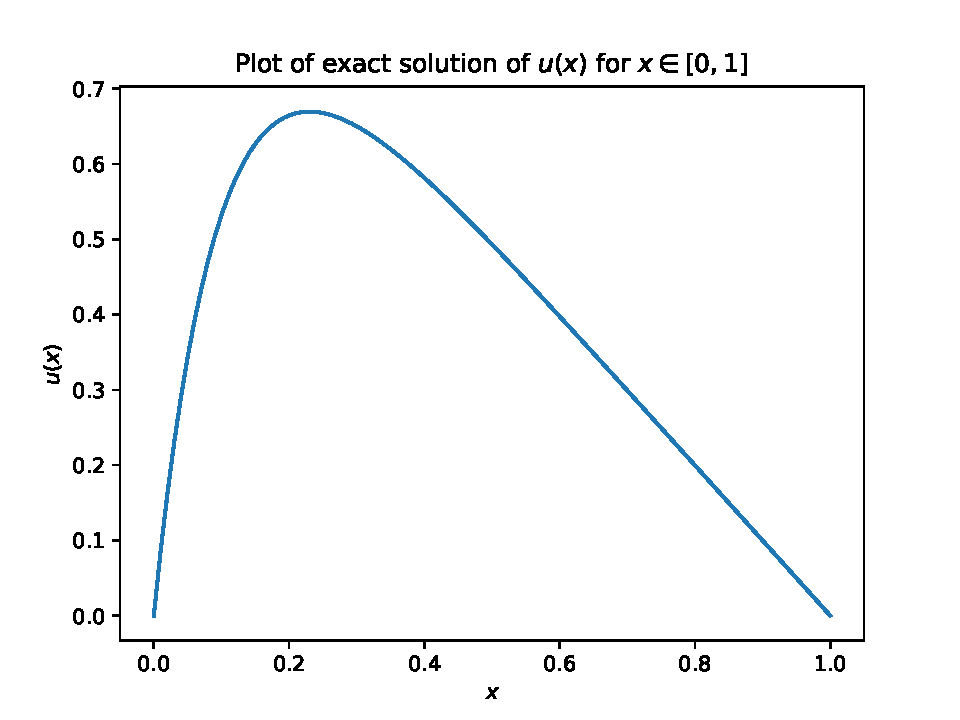
\includegraphics[scale=0.80]{../data/exactSolution.pdf} %Imports the figure.
    \caption{Plot of the exact solution of $u(x)$ for $x ∈ [0,1]$. We used $n =100$ data points for the plot.}
    \label{plot_problem2}
\end{figure}


\section*{Problem 3}
Our aim is to derive a discretized version of the Poisson equation which lets us calculate approximates values $v$ of the exact values $u$. To create this program we need to discretize the double derivative, which we can do by recalling its definition:
\begin{equation}
    \frac{\text{d}^2u}{\text{d}u^2} = \lim_{\text{d}x\to 0}\frac{-u(x -\text{d}x) + 2u(x) - u(x + \text{d}x)}{\text{d}x^2} 
\end{equation}
If we let the infinitesimal value $\text{d}x$ rather become a finite, small value $\Delta x$, we'll still be able to calculate the double derivative with good precision, as long as we don't let this value grow too large. Since this is an approximation, a discretized version of \cref{poisson}, we will use $v(x)$ instead of $u(x)$ in the following procedures to make it clear that this is not an exact solution. The resulting equation becomes
\begin{equation}
    \frac{-v(x -\Delta x) + 2v(x) - v(x + \Delta x) }{\Delta x^2} = -100e^{-10x} 
\end{equation}
Let's denote the $i^\text{th}$ $x$-value in out set of data points with $x_i$, so that the corresponding $v$-value will be denoted with $v_i$. This implies that at the boundaries we have $x_0 = 0$, $v_0 = 0$, and $x_{N-1} = 1$, $v_{N-1} = 0$, where $N$ are the number of data points. Thus, the final algorithm is
\begin{equation}
    \frac{-v_{i-1} + 2v_i - v_{i+1}}{h^2} = f_i \label{discretized poisson}
\end{equation}
where $h = \Delta x$ is defined as
\begin{equation}
    h = \frac{x_N - x_0}{N-1}
\end{equation}
and we've rewritten the forcing term to include the minus sign that was originally on the left hand side of the equation, meaning that
\begin{equation}
    f_i = f(x_i) = -100e^{-10x_i}
\end{equation}


\section*{Problem 4}
Let us now multiply $h^2$ with both sides of \cref{discretized poisson}, consequently rewriting the equation:
\begin{equation}
    -v_{i-1} + 2v_i - v_{i+1} = g_i, \hspace{15pt} g_i = h^2f_i \label{g_i define}
\end{equation}
Furthermore, we may define the vectors $\vec{v}$ and $\vec{g}$ such that
\begin{equation}
    \vec{v} = \begin{bmatrix}
        v_0 \\
        v_1 \\
        \vdots \\
        v_{N-1}
    \end{bmatrix}, \hspace{15pt} \vec{g} = \begin{bmatrix}
        g_0 \\
        g_1 \\
        \vdots \\
        g_{N-1}
    \end{bmatrix}
\end{equation}

Using our knowledge of linear algebra, we may now define the matrix
\begin{equation}
    \textbf{A} = \begin{bmatrix}
        2 & -1 & 0 & \ldots & 0 \\
        -1 & 2 & -1 & \ldots & \vdots \\
        0 & -1 & 2 & \ldots & \vdots \\
        \vdots&\vdots&\vdots&\ddots & \vdots \\
        0 & \ldots&\ldots & \ldots & 2
    \end{bmatrix}
\end{equation}
which multiplied with $\vec{v}$ gives us
\begin{equation}
    \textbf{A}\vec{v} = \begin{bmatrix}
        2 & -1 & \ldots & 0 \\
        -1 & 2 & \ldots & \vdots \\
        \vdots&\vdots&\ddots&\vdots \\
        0 & \ldots & \ldots & 2
    \end{bmatrix} \begin{bmatrix}
        v_0 \\
        v_1 \\
        \vdots \\
        v_{N-1}
    \end{bmatrix} = \begin{bmatrix}
        2v_0 - v_1 \\
        -v_0 + 2v_1 -v_2 \\
        \vdots\\
        -v_{N-2}+2v_{N-1}
    \end{bmatrix}
\end{equation}

We immediately see from \cref{g_i define} that this gives us the vector $\vec{g}$ containing the $g_i$-values with the same indexes as the corresponding $v_i$-values from $\vec{v}$. Thus, we can indeed rewrite the original discretized equation as the matrix equation
\begin{equation}
    \textbf{A}\vec{v} = \vec{g} \label{matrix eq}
\end{equation}
where $\textbf{A}$ is the tridiagonal matrix with subdiagonal, main diagonal and superdiagonal specified by the signature $(-1, 2, -1)$, just like we wanted to show.


\section*{Problem 5}
\subsection*{Problem 5a}
We now have the vectors $\vec{v}^*$ and $\vec{x}$, both of length $m$, and the matrix $\text{bf}$ of size $n \times n$. This means that we have $m$ number of data points, and that if we wish to solve \cref{matrix eq} with the matrix $\textbf{A}$ we can only solve for $n$ of the data points. This is because we never can multiply a matrix with a vector if the matrix has more or less columns than the amount of elements the vector has. Thus, the number $n$ indicates how many of the values in the complete solution we will be able to calculate by solving the equation.

\subsection*{Problem 5b}
If $n < m$ we will only be able to compute the first $n$ elements in the complete solution $\vec{v}^*$, or alternatively the last $n$ elements if we use the last $n$ elements in $\vec{x}$ to compute the elements in $\vec{g}$.


\section*{Problem 6}
\subsection*{Problem 6a}
Now we consider the general tridiagonal matrix with subdiagonal, main diagonal and superdiagonal represented by the vectors $\vec{a}$, $\vec{b}$ and $\vec{c}$, respectively. Such a matrix would have the from
\begin{equation}
    \textbf{A} = \begin{bmatrix}
        b_0 & c_0 & 0 & \ldots & 0 \\
        a_0 & b_1 & c_1 & \ldots & \vdots\\
        0 & a_1 & b_2 & \ldots & \vdots\\
        \vdots&\vdots&\vdots&\ddots&\vdots\\
        0 & \ldots & \ldots & a_{n-2} & b_{n-1} 
    \end{bmatrix}
\end{equation}
should its dimensions be $n \times n$. To study the general algorithm of computing \cref{matrix eq}, let us look at the case of $n = 3$. If we augment $\vec{g}$ to $\textbf{A}$ so that we get
\begin{equation}
    \left[\textbf{A }\vec{g}\right] = \begin{bmatrix}
        b_0 & c_0 & 0 & g_0 \\
        a_0 & b_1 & c_1 & g_1 \\
        0 & a_1 & b_2 & g_2 
    \end{bmatrix}
\end{equation}
we can use the Gaussian elimination method to turn the part of the matrix that is originally just $\textbf{A}$ into the identity matrix. We could either use forward substitution or backwards substitution to go further, so let's try using the former. First, we can multiply row I of the augmented matrix with $a_0/b_0$ and then subtract that row from row II:
\begin{equation}
    \begin{bmatrix}
        b_0 & c_0 & 0 & g_0 \\
        0 & b_1 - a_0c_0/b_0 & c_1 & g_1 - a_0g_0/b_0 \\
        0 & a_1 & b_2 & g_2 
    \end{bmatrix}
\end{equation}
To make the calculations more readable, let's introduce the new variables $\overline{b}_1 = b_1 - a_0c_0/b_0$ and $\overline{g}_1 = b_1 - a_0g_0/b_0$. Furthermore, let's now multiply row II with $a_1/\overline{b}_1$ and subtract it from row III so that we're left with
\begin{equation}
    \begin{bmatrix}
        b_0 & c_0 & 0 & g_0 \\
        0 & \overline{b}_1 & c_1 & \overline{g}_1 \\
        0 & 0 & b_2 - a_1c_1/\overline{b}_1 & g_2 - a_1\overline{g}_1/\overline{b}_1
    \end{bmatrix}
\end{equation}
Once again we introduce some new variables, $\overline{b}_2 = b_2 - a_1c_1/\overline{b}_1$ and $\overline{g}_2 = g_2 - a_1\overline{g}_1/\overline{b}_1$. Dividing row III with $\overline{b}_2$ we're then left with
\begin{equation}
    \begin{bmatrix}
        b_0 & c_0 & 0 & g_0 \\
        0 & \overline{b}_1 & c_1 & \overline{g}_1 \\
        0 & 0 & 1 & v_2
    \end{bmatrix}
\end{equation}
What we're left with on the bottom left is now actually the third value in the solution to the original equation. To find $v_2$ and $v_1$ we work our way upward with similar calculations. First we multiply row III with $c_1$ and subract it from row II, then we divide row II with $b_1$ so that we have $1$ on the diagonal element on row II. Finally we multiply row II with $c_0$ and subtract it from row I, then dividing row I with $b_0$ so that we're left with
\begin{equation}
    \begin{bmatrix}
        1 & 0 & 0 & v_0 \\
        0 & 1 & 0 & v_1 \\
        0 & 0 & 1 & v_2
    \end{bmatrix}
\end{equation}
As we can see we're now left with the vector $\vec{v}$ that would satisfy \cref{matrix eq} in column IV. This process is analogous for any equation where $\textbf{A}$ is an $m \times n$ matrix, $\vec{v}$ is a vector of size $n$ and $\vec{g}$ is a vector of size $m$. A general pseudo code of this process when $\textbf{A}$ is a tridiagonal matrix could look like in \cref{algorithm matrix eq}. Here it is assumed that one would first create a new matrix $\textbf{A}g$ that is a copy of $\textbf{A}$ with $\vec{g}$ concatenated to it.

\begin{algorithm}[H]
    \caption{Pseudo code for solving $\textbf{A}\vec{v} = \vec{g}$ for $\vec{v}$}\label{algorithm matrix eq}
    \begin{algorithmic}
        \For{$i = 0, 1, ..., n-2$} \Comment{in this loop we get rid of the subdiagonal in the augmented matrix}
        \State $newrow = \textbf{A}g[i]\textbf{A}g[i+1,i] / \textbf{A}g[i,i];$ 
        \State $\textbf{A}g[i+1] = \textbf{A}g[i+1] - newrow;$ \Comment{$a_i = 0$, $b_{i+1} = b_{i+1} - c_i a_i / b_i$ and $g_{i+1} = g_{i+1} - g_ia_i / b_i$}
        \EndFor
        \State
        \For{$i = n-1, n-2, ..., 1$} \Comment{in this loop we get rid of the superdiagonal and normalize the diagonal elements}
        \State $\textbf{A}g[i] = \textbf{A}g[i] / \textbf{A}g[i,i];$ \Comment{$v_i = \overline{g}_i/\overline{b}_i$}
        \State $\textbf{A}g[i-1] = \textbf{A}g[i-1] - \textbf{A}g[i-1,i]\textbf{A}g[i];$ \Comment{$v_{i-1} = v_{i-1} - c_{i-1}v_i$}
        \EndFor
        \State
        \State $\triangleright$ lastly we impose the boundary conditions
        \State $\textbf{A}g[0,n] = 0.0;$ \Comment{$v_0 = 0.0$} 
        \State $\textbf{A}g[n-1,n] = 0.0;$ \Comment{$v_{n-1} = 0.0$} 
    \end{algorithmic}
\end{algorithm}

\subsection*{Problem 6b}
In \cref{algorithm matrix eq} we do two FLOPs to three nonzero matrix elements in the first line of the first loop, and then do one FLOP to three matrix elements in the next line. Since we do this $n-1$ times, this loop contains a total amount of $(2*3)(n-1) + 3(n-1) = 9(n-1)$ FLOPs. In the next loop we do one FLOP to two nonzero matrix elements in the first line, while in the second line we do one FLOP to two nonzero matrix elements and one FLOP to two other nonzero matrix elements. Since we do this $n-1$ times as well, this loop contains a total of $2(n-1) + 2(n-1) + 2(n-1) = 6(n-1)$ FLOPs. Thus, the algorithm contains $15(n-1)$ FLOPs. However, in order to apply this algorithm to our program, we had to use vectors instead of matrices because the matrices take up too much storage for sufficiently large values of $n$. To further optimalize our code we only operated with the vector elements different from zero, instead of operating with the entire row vectors. Thus, we ended up using \cref{algorithm fixed}. In this algorithm we do six FLOPs in the first loop, which we do $n-1$ times, and in the second loop we do three FLOPs, which we also do $n-1$ times. Thus, the optimalized algorithm contains $9(n-1)$ FLOPs.

\section*{Problem 7}
\subsection*{Problem 7a}
When implementing \cref{algorithm matrix eq} in C++, we quickly stumbled into a memory issue. To run this algorithm for $n=10^7$ we would need to create a matrix of size $10^7 \times 10^7$, which would require $10^7 \times 10^7 \times 8 = 8 × 10^{14}$ bytes of memory when using doubles. This is equal to 800 TB, which is more than the amount of memory on the computers we're using. Thus, we needed to find a way to solve this problem without creating such a large matrix. Looking at the algorithim, we notice we only needed to calculate two rows at a time. Therefore, we could use the armadillo library to store the two rows as vectors. This allowed us to solve the problem, but this approach was still quite slow. We calculated a runtime of approximately 8-16 hours with this approach. Finally we noticed that we don't need to store the entire rows, only the nonzero elements in two rows at a time. This pattern is easy to see in the case of $n=5$ as seen in \cref{fig: vector_example}. In the first loop, we only use index 1, 2 and $n$ in row 1, and index 2, 3, $n$ in row 2. In the second loop, row 1 replaces row 2 and the indexes of interest in row 2 increase by one. To copy over $n$ elements is computationally heavy and a foor-loop in of itself. By noticing the fact that there are only three indices of interest, we can store just 3 values instead of $n$. This reduces the time complexity from $O(n^2)$ to $O(n)$ and increased computation speed by a factor of 125'000-250'000.

The final function we wrote which implemented the general algorithm is found in the file \verb|find_v_general.cpp|. In \verb|main.cpp| we call on this function for $n_\text{steps} = 10, 100, 1000, 10^4, 10^5, 10^6, 10^7$. We also call on the function \verb|write_to_file| for each of these values of $n_\text{steps}$ to store the solutions $\vec{v}$ and the corresponding vectors $\vec{x}$ to binary files. We chose to write the data to binary files to save time.

\begin{figure}
    \centering
    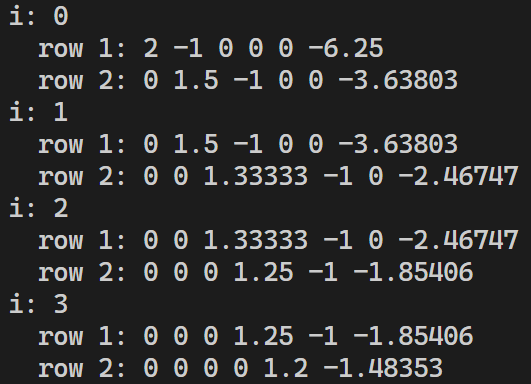
\includegraphics[scale=0.5]{vector_example.png}
    \caption{Screenshot of terminal output showing calculations for $n = 5$}
    \label{fig: vector_example}
\end{figure}

\subsection*{Problem 7b}
After running our program for all the seven values of $n_\text{steps}$ we used our script \verb|plot_data.py| to plot the numerical solutions along with the exact solution $u(x)$. The resulting plot is shown in \cref{plot7b}. In \cref{plot7b w/o 10} we plotted the numerical solutions without the one corresponding to $n_\text{steps} = 10$, as this one deviated so much that it was difficult to decipher the precision of the other solutions.

\begin{algorithm}[H]
    \caption{Optimalized pseudo code for solving $\textbf{A}\vec{v} = \vec{g}$ for $\vec{v}$}\label{algorithm fixed}
    \begin{algorithmic}
        \State $\triangleright$ before the first loop we specify the nonzero elements of the first row in the augmented matrix, denoted $\textbf{A}g_0$
        \State $\textbf{A}g_{0,0} = b[0]$; \Comment{first element in first row is $b_0$}
        \State $\textbf{A}g_{0,1} = c[0]$; \Comment{second element in first row is $c_0$}
        \State $\textbf{A}g_{0,n} = g[0]$; \Comment{last element in first row is $g_0$}
        \State
        \For{$i = 0, 1, ..., n-2$} \Comment{in this loop we get rid of the subdiagonal in the augmented matrix}
        \State $\triangleright$ here we specify the nonzero elements of row no. $i+1$, denoted $\textbf{A}g_{i+1}$
        \State $\textbf{A}g_{i+1,i} = a[i]$; \Comment{$i$'th element in row no. $i+1$ is $a_i$}
        \State $\textbf{A}g_{i+1,i+1} = b[i+1]$; \Comment{$(i+1)$'th element in row no. $i+1$ is $b_{i+1}$}
        \If{$i < n-2$} \Comment{on the last row we don't have any $c$-value}
        \State $\textbf{A}g_{i+1,i+2} = c[i+1]$; \Comment{$(i+2)$'th element in row no. $i+1$ is $c_{i+1}$}
        \EndIf
        \State $\textbf{A}g_{i+1,n} = g[i+1]$; \Comment{$n$'th element in row no. $i+1$ is $g_{i+1}$}
        \State
        \State $\triangleright$ here we perform the matrix operations between row $\textbf{A}g_{i}$ and row $\textbf{A}g_{i+1}$ only on the nonzero row elements
        \State $\textbf{A}g_{i+1,i+1} = \textbf{A}g_{i+1,i+1} - \textbf{A}g_{i,i+1} \textbf{A}g_{i+1,i} / \textbf{A}g_{i,i}$; \Comment{$b_{i+1} = b_{i+1} - c_i a_i / b_i$}
        \State $\textbf{A}g_{i+1,n} = \textbf{A}g_{i+1,n} - \textbf{A}g_{i,n} \textbf{A}g_{i+1,i} / \textbf{A}g_{i,i};$ \Comment{$g_{i+1} = g_{i+1} - g_ia_i / b_i$}
        \State $\textbf{A}g_{i+1,i} = 0.0$; \Comment{$a_i = a_i - b_ia_i/b_i = 0$}
        \State
        \State $\triangleright$ here we store the modified diagonal element and the modified $g_i$ for the next loop
        \State $diag[i] = \textbf{A}g_{i,i}$; \Comment{stores $\overline{b}_{i}$ for later use}
        \State $v[i] = \textbf{A}g_{i,n}$; \Comment{stores $\overline{g}_{i}$ for later use}
        \State
        \State $\triangleright$ here we essentially want to replace row $\textbf{A}g_{i}$ with row $\textbf{A}g_{i+1}$ for the next operations
        \State $\textbf{A}g_{i,i} = \textbf{A}g_{i+1,i+1}$; \Comment{replaces $\overline{b}_i$ with $b_{i+1}$ }
        \State $\textbf{A}g_{i,i+1} = \textbf{A}g_{i+1,i+2}$; \Comment{replaces $c_i$ with $c_{i+1}$ }
        \State $\textbf{A}g_{i,n} = \textbf{A}g_{i+1,n}$; \Comment{replaces $\overline{g}_i$ with $g_{i+1}$}
        \EndFor
        \State
        \State $\triangleright$ the $(i+1)$'th row is now the last row, so we store the nonzero values from this row in $diag$ and $v$
        \State $diag[n-1] = \textbf{A}g_{i+1,i}$; \Comment{stores $\overline{b}_{n-1}$ for later use} 
        \State $v[n-1] = \textbf{A}g_{i+1,n}$; \Comment{stores $\overline{g}_{n-1}$ for later use}
        \State
        \For{$i = n-1, n-2, ..., 1$} \Comment{in this loop we get rid of the superdiagonal and normalize the diagonal elements}
        \State $v[i] = v[i]/diag[i]$; \Comment{$v_{i} = \overline{g}_i/\overline{b}_i$} 
        \State $v[i-1] = v[i-1] - c[i-1]v[i]$; \Comment{$v_{i-1} = v_{i-1} - c_{i-1}v_{i}$}
        \EndFor
        \State
        \State $\triangleright$ lastly we impose the boundary conditions
        \State $v[0] = 0.0$; \Comment{$v_0 = 0.0$} 
        \State $v[n-1] = 0.0$; \Comment{$v_{n-1} = 0.0$} 
        
    \end{algorithmic}
\end{algorithm}

\subsection*{Problem 7b}
After running our program for all the seven values of $n_\text{steps}$ we used our script \verb|plot_data.py| to plot the numerical solutions along with the exact solution $u(x)$. The resulting plot is shown in \cref{plot7b}. In \cref{plot7b w/o 10} we plotted the numerical solutions without the one corresponding to $n_\text{steps} = 10$, as this one deviated so much that it was difficult to decipher the precision of the other solutions.

\begin{figure}[h!]
    \centering 
    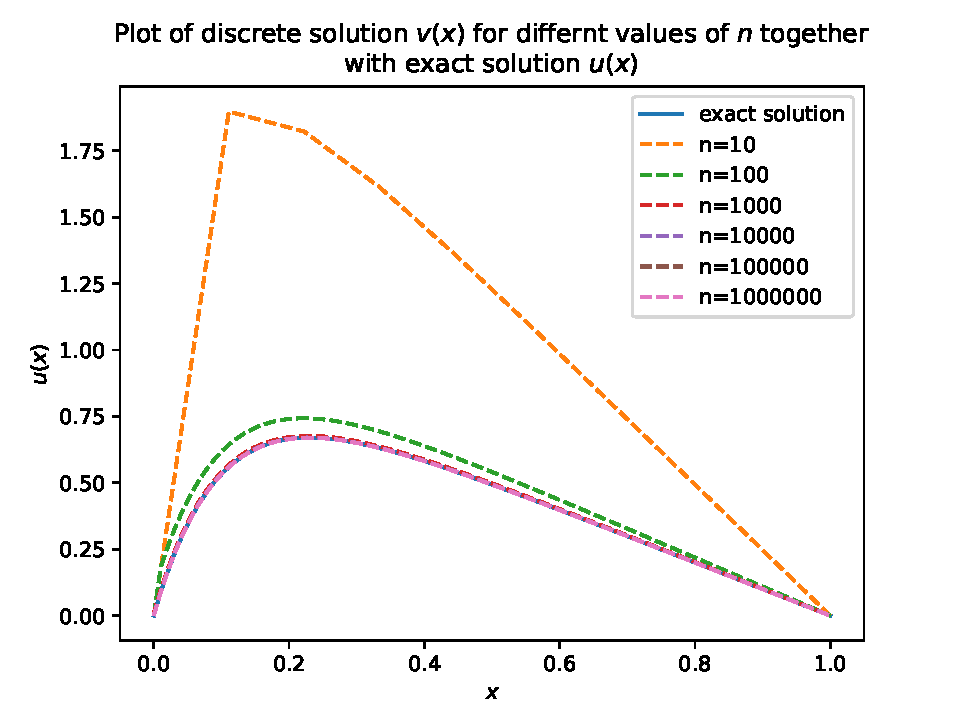
\includegraphics[scale=0.80]{/Users/paljettrosa/Documents/GitHub/FYS3150-ComputationalPhysics/Project1/data/exactVSdiscrete.pdf} %Imports the figure.
    \caption{Plot of the numerical solutions $v(x)$ for seven different values of $n_\text{step}$ (dashed lines) along with the exact solution $u(x)$ (solid line).}
    \label{plot7b}
\end{figure}

\begin{figure}[h!]
    \centering 
    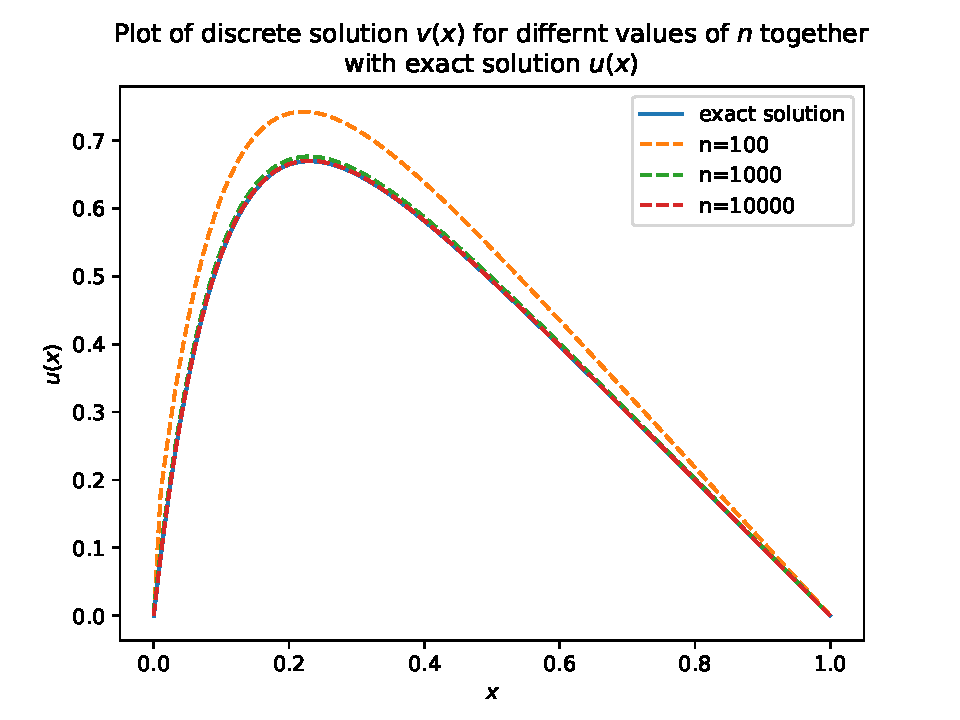
\includegraphics[scale=0.80]{/Users/paljettrosa/Documents/GitHub/FYS3150-ComputationalPhysics/Project1/data/exactVSdiscrete_wo10.pdf} %Imports the figure.
    \caption{Plot of the numerical solutions $v(x)$ (dashed lines) without $n_\text{step} = 10$ along with the exact solution $u(x)$ (solid line).}
    \label{plot7b w/o 10}
\end{figure}

\section*{Problem 8}
\subsection*{Problem 8a}
In \cref*{abs err} we see a plot of the logarithm of the absolute errors 
\begin{equation}
    \log_{10}(\Delta_i) = \log_{10}(|u_i - v_i|)
\end{equation}
of the numerical solutions as functions of $x_i$ for the seven different values of $n_\text{step}$.

\begin{figure}[h!]
    \centering 
    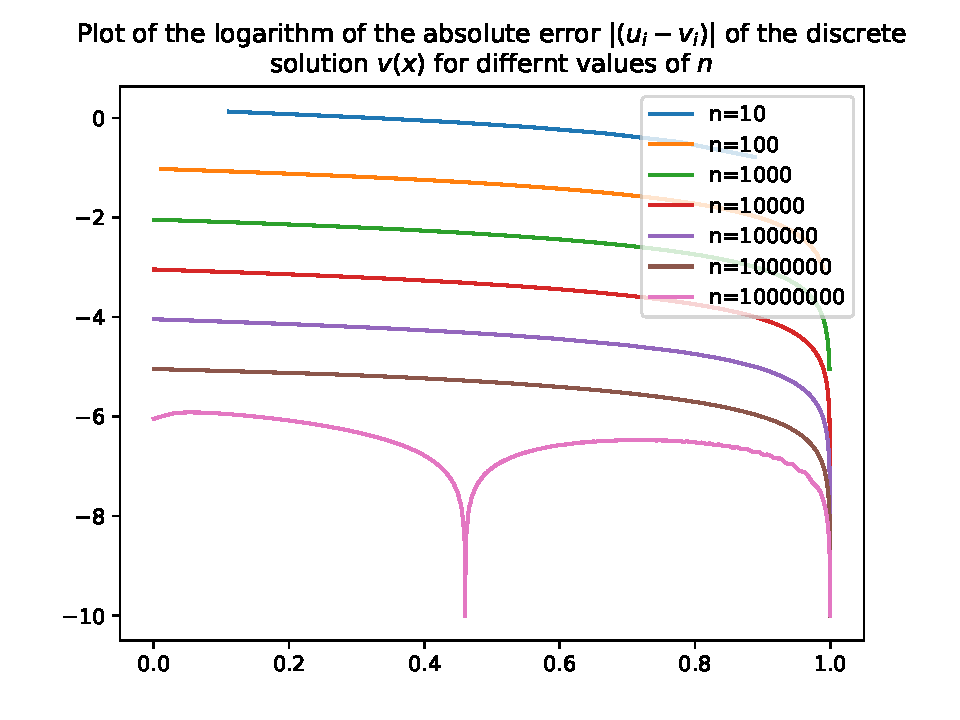
\includegraphics[scale=0.80]{/Users/paljettrosa/Documents/GitHub/FYS3150-ComputationalPhysics/Project1/data/absolute_error.pdf} %Imports the figure.
    \caption{Plot of the logarithm of the numerical solutions' absolute errors $\log_{10}(\Delta_i)$ $v(x)$ for the seven different values of $n_\text{step}$.}
    \label{abs err}
\end{figure}

\subsection*{Problem 8b}
In \cref{rel err} we instead see a plot of the logarithm of the relative errors 
\begin{equation}
    \log_{10}(\epsilon_i) = \log_{10}\left(\left|\frac{u_i - v_i}{u_i}\right|\right)
\end{equation}
of the numerical solutions as functions of $x_i$ for the seven different values of $n_\text{step}$.

\begin{figure}[h!]
    \centering 
    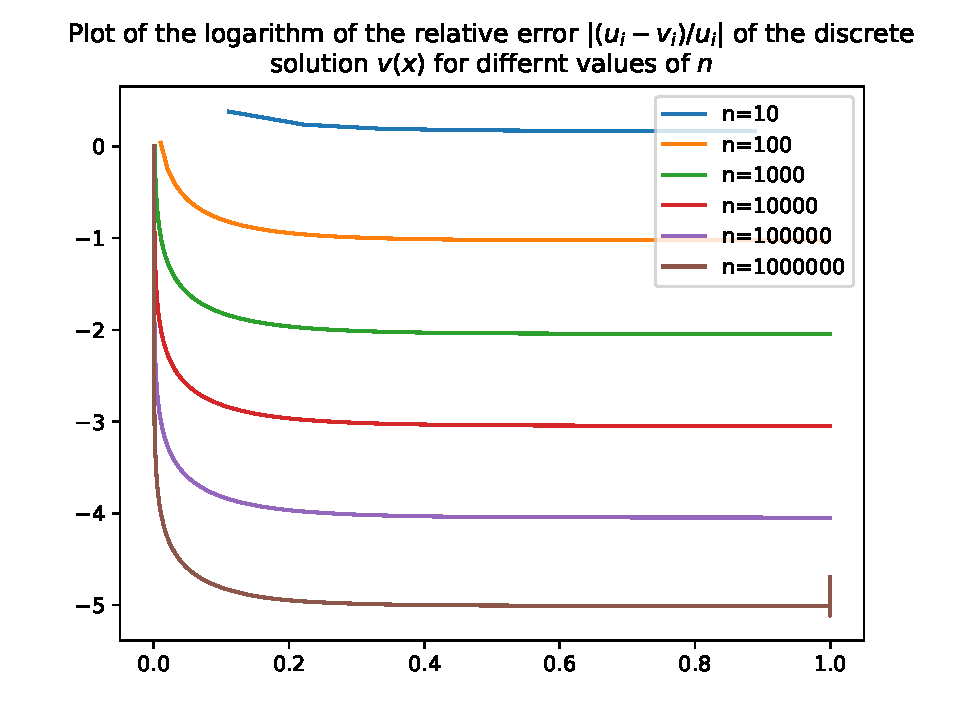
\includegraphics[scale=0.80]{/Users/paljettrosa/Documents/GitHub/FYS3150-ComputationalPhysics/Project1/data/relative_error.pdf} %Imports the figure.
    \caption{Plot of the logarithm of the numerical solutions' relative errors $\log_{10}(\epsilon_i)$ $v(x)$ for the seven different values of $n_\text{step}$.}
    \label{rel err}
\end{figure}

\subsection*{Problem 8c}
Table \ref{max rel err} shows the maximum relative errors of the numerical solutions for the seven values of $n_\text{steps}$, along with the corresponding $x$-values where the errors were largest. We see that the errors are largest near $x = 0$, but naturally not at $x = 0$ since we set the first and last values of $\vec{v}$ to zero. This is not surprising considering the plot of the logarithm of the relative errors, as these all peak near $x = 0$ This is due to the fact that we divide by $u_i$ when calculating $\epsilon_i$, and the first $u_i$ are very close to zero, as well as $u_i - v_i$ being close to zero.
\begin{table}%[h!]
    \centering
    \caption{Table showing the maximum relative error $\text{max}(\epsilon_i)$ of the numerical solutions along with the corresponding $x$-values $x_i$, for seven values of $n_\text{step}$.}
    \begin{tabular}{c@{\hspace{1cm}} c@{\hspace{1cm}} c}
        \hline
        $n_\text{steps}$ & $\text{max}(\epsilon_i)$ & $x_i$ \\
        \hline
        10\hspace{4pt} & 2.390320018853711 & 0.1111111111\\
        $10^2$ & 1.094617632100603 & 0.0101010101 \\
        $10^3$ & 1.0091451046464817 & 0.001001001 \\
        $10^4$ & 1.0009115217009974 & 0.00010001 \\
        $10^5$ & 1.0000900036001439 & 1.00001$\times 10^{-05}$ \\
        $10^6$ & 1.0000111111111112 & $10^{-6}$ \\
        $10^7$ & 1.0 & $10^{-7}$ \\
        \hline
    \end{tabular}\label{max rel err}
\end{table}


\section*{Problem 9}
\subsection*{Problem 9a}
To specialize our algorithm from Problem 6 where $\textbf{A}$ is specified by the signature $(-1, 2, -1)$ we essentially used the general algorithm. The only difference is that the function \verb|find_v_special| we created that is defined in \verb|find_v_special.cpp| doesn't take in vectors $\vec{a}$, $\vec{b}$ and $\vec{c}$. Instead the constant doubles $a = -1.0$, $b = 2.0$ and $c =-1.0$ are defined locally within the function.

\subsection*{Problem 9b}
The special algorithm contains the exact same number of FLOPs as the general algorithm, which is $9(n-1)$.

\subsection*{Problem 9c}
See \verb|find_v_special.cpp|.


\section*{Problem 10}
Figures \ref{timing 1}, \ref{timing 2}, \ref{timing 3}, \ref{timing 4}, \ref{timing 5} and \ref{timing 6} show comparisons of fice runtimes with the general algorithm and the special algorithm for $n_\text{steps} = 10, 100, 1000, 10^4, 10^5, 10^6$ respectively. The diagrams also compare the mean of the five runtimes in each case. As expected, considering there is an equal amount of FLOPs in them both, there are minor differences between the two algorithms, and these may very well be random. It does however seem like the general algorithm tends to be somewhat slower than the special algorithm, which may have something to do with the fact that the general algorithm picks out elements from the vectors $\vec{a}$, $\vec{b}$ and $\vec{c}$ before performing computations.

\begin{figure}[h!]
    \vspace*{20pt}
    \centering 
    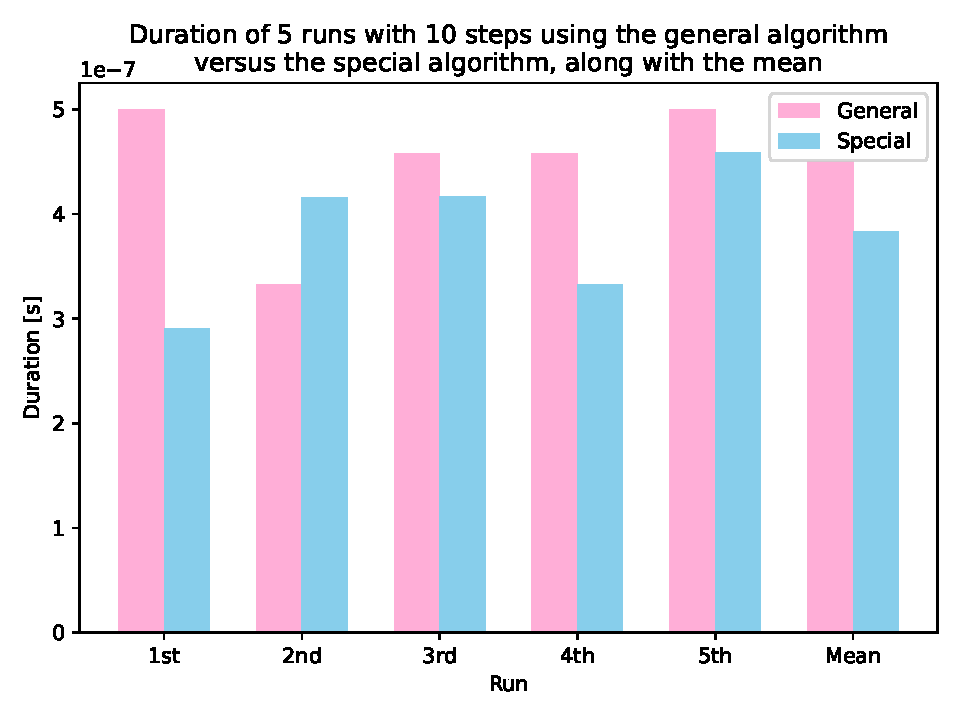
\includegraphics[scale=0.80]{/Users/paljettrosa/Documents/GitHub/FYS3150-ComputationalPhysics/Project1/data/runtime_comparison_10.pdf} %Imports the figure.
    \caption{Comparison of runtimes for $n_\text{step} = 10$ from five seperate runs as well as the mean of these using the general algorithm (pink) and special algorithm (blue).}
    \label{timing 1}
\end{figure}

\begin{figure}[h!]
    \centering 
    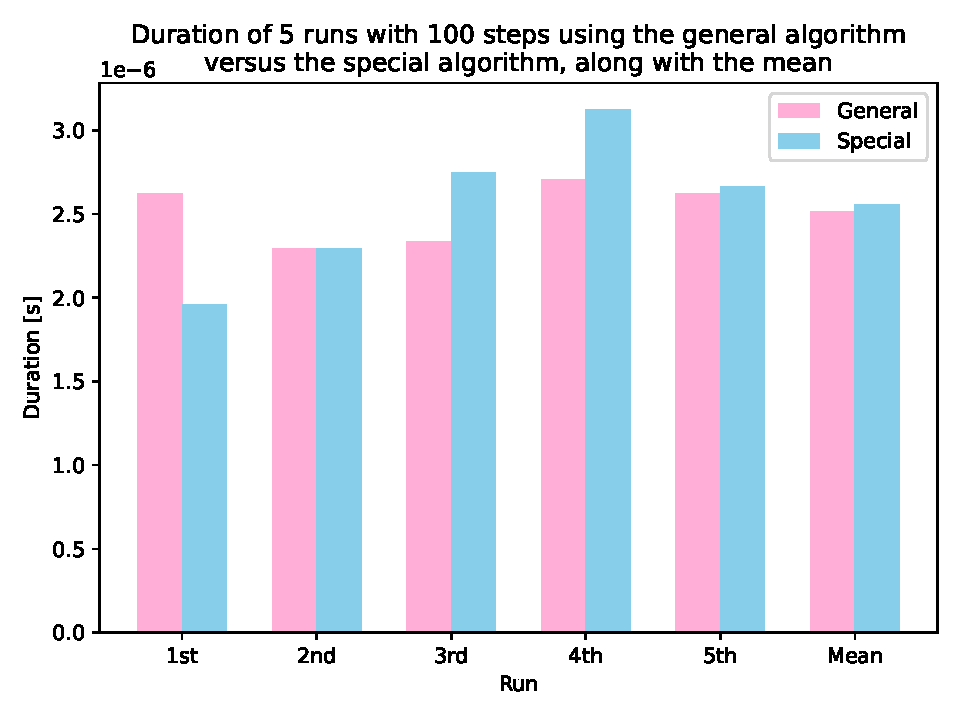
\includegraphics[scale=0.80]{/Users/paljettrosa/Documents/GitHub/FYS3150-ComputationalPhysics/Project1/data/runtime_comparison_100.pdf} %Imports the figure.
    \caption{Comparison of runtimes for $n_\text{step} = 100$ from five seperate runs as well as the mean of these using the general algorithm (pink) and special algorithm (blue).}
    \label{timing 2}
\end{figure}

\begin{figure}[h!]
    \centering 
    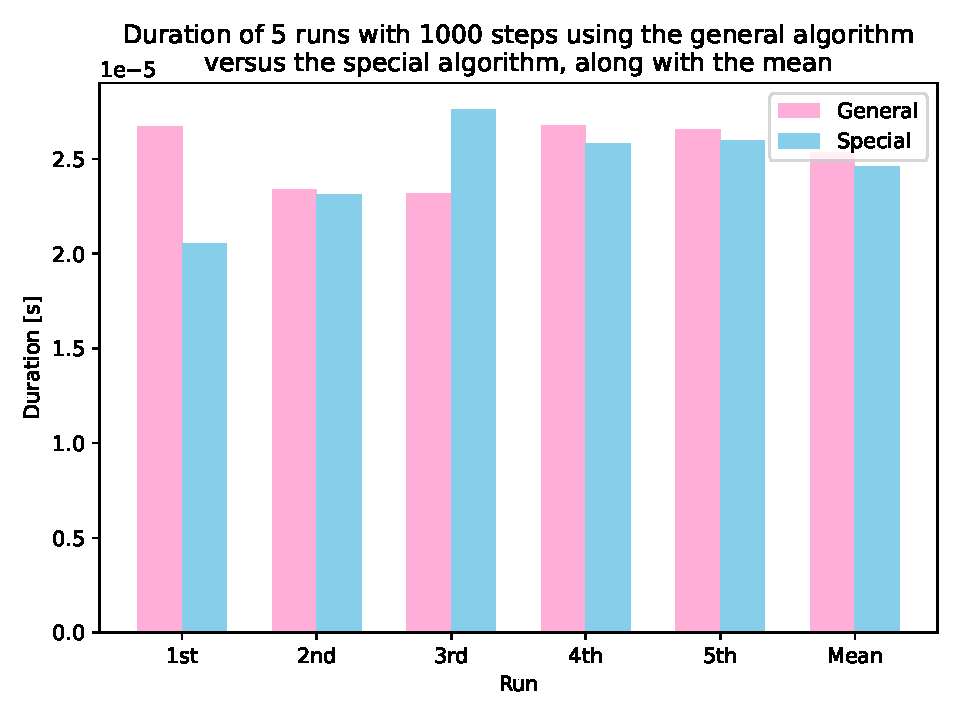
\includegraphics[scale=0.80]{/Users/paljettrosa/Documents/GitHub/FYS3150-ComputationalPhysics/Project1/data/runtime_comparison_1000.pdf} %Imports the figure.
    \caption{Comparison of runtimes for $n_\text{step} = 1000$ from five seperate runs as well as the mean of these using the general algorithm (pink) and special algorithm (blue).}
    \label{timing 3}
\end{figure}

\begin{figure}[h!]
    \centering 
    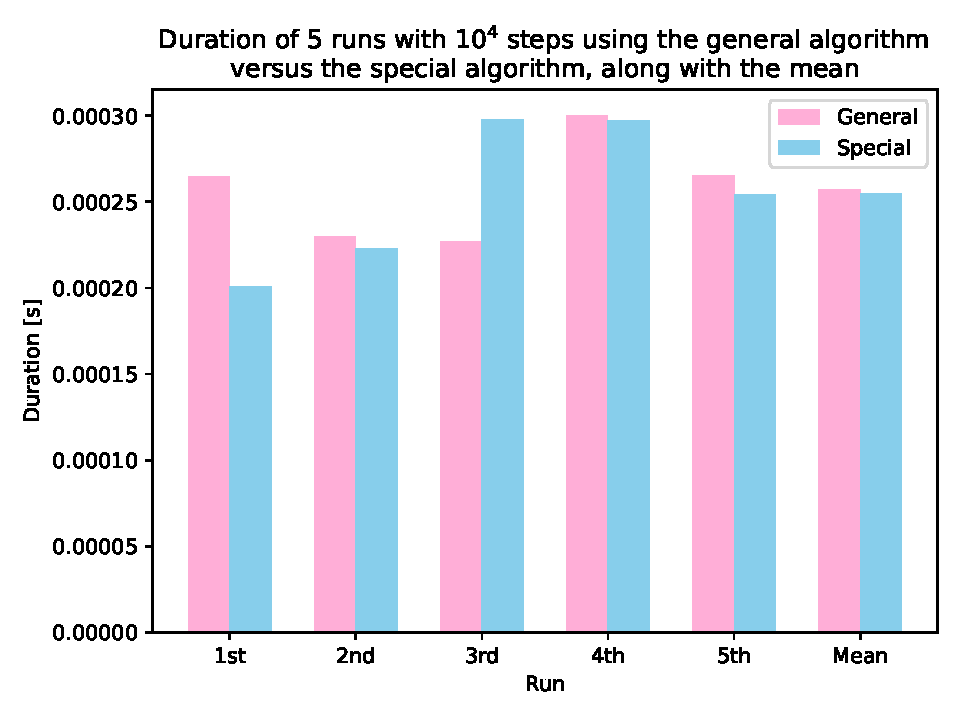
\includegraphics[scale=0.80]{/Users/paljettrosa/Documents/GitHub/FYS3150-ComputationalPhysics/Project1/data/runtime_comparison_10000.pdf} %Imports the figure.
    \caption{Comparison of runtimes for $n_\text{step} = 10^4$ from five seperate runs as well as the mean of these using the general algorithm (pink) and special algorithm (blue).}
    \label{timing 4}
\end{figure}

\begin{figure}[h!]
    \centering 
    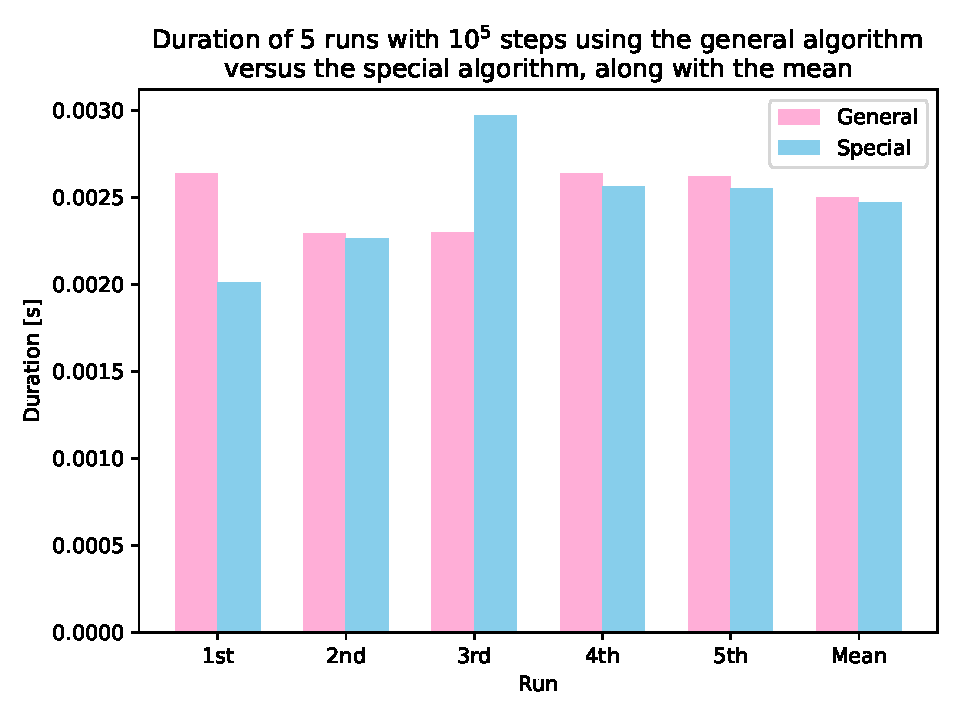
\includegraphics[scale=0.80]{/Users/paljettrosa/Documents/GitHub/FYS3150-ComputationalPhysics/Project1/data/runtime_comparison_100000.pdf} %Imports the figure.
    \caption{Comparison of runtimes for $n_\text{step} = 10^5$ from five seperate runs as well as the mean of these using the general algorithm (pink) and special algorithm (blue).}
    \label{timing 5}
\end{figure}

\begin{figure}[h!]
    \centering 
    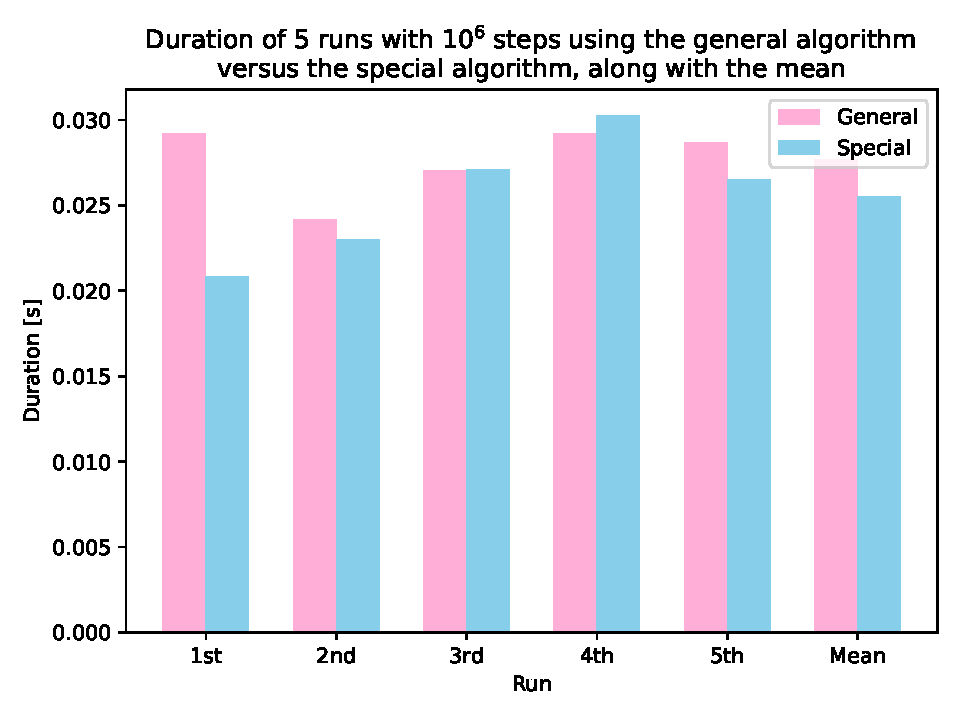
\includegraphics[scale=0.80]{/Users/paljettrosa/Documents/GitHub/FYS3150-ComputationalPhysics/Project1/data/runtime_comparison_1000000.pdf} %Imports the figure.
    \caption{Comparison of runtimes for $n_\text{step} = 10^6$ from five seperate runs as well as the mean of these using the general algorithm (pink) and special algorithm (blue).}
    \label{timing 6}
\end{figure}

   
\end{document}
